\documentclass[11pt]{article}
\usepackage{geometry,marginnote} % Pour passer au format A4
\geometry{hmargin=1cm, vmargin=1.5cm} % 

% Page et encodage
\usepackage[T1]{fontenc} % Use 8-bit encoding that has 256 glyphs
\usepackage[english,french]{babel} % Français et anglais
\usepackage[utf8]{inputenc} 

\usepackage{lmodern}
\usepackage[np]{numprint}
\setlength\parindent{0pt}

% Graphiques
\usepackage{graphicx,float,grffile}
\usepackage{tikz,pst-eucl,pst-plot,pstricks,pst-node,pstricks-add,pst-fun,pgfplots} 

% Maths et divers
\usepackage{amsmath,amsfonts,amssymb,amsthm,verbatim,scratch3}
\usepackage{multicol,enumitem,url,eurosym,gensymb,tabularx}

\DeclareUnicodeCharacter{20AC}{\euro}



% Sections
\usepackage{sectsty} % Allows customizing section commands
\allsectionsfont{\centering \normalfont\scshape}

% Tête et pied de page
\usepackage{fancyhdr} \pagestyle{fancy} \fancyhead{} \fancyfoot{}

%\fancyfoot[L]{Collège Faubert}
%\fancyfoot[C]{\thepage / 6}
%\fancyfoot[R]{Série Générale}

\renewcommand{\headrulewidth}{0pt} % Remove header underlines
%\renewcommand{\footrulewidth}{0pt} % Remove footer underlines

\newcommand{\horrule}[1]{\rule{\linewidth}{#1}} % Create horizontal rule command with 1 argument of height

\newcommand{\Pointilles}[1][3]{%
  \multido{}{#1}{\makebox[\linewidth]{\dotfill}\\[\parskip]
}}

\newtheorem{Definition}{Définition}

\usepackage{siunitx}
\sisetup{
    detect-all,
    output-decimal-marker={,},
    group-minimum-digits = 3,
    group-separator={~},
    number-unit-separator={~},
    inter-unit-product={~}
}

\setlength{\columnseprule}{1pt}


\begin{document}
\textbf{Nom, Prénom :} \hspace{8cm} \textbf{Classe :} \hspace{3cm} \textbf{Date :}\\

\begin{center}
  \textit{Le plus grand ennemi de la connaissance n'est pas l'ignorance. C'est l'illusion de la connaissance.} 
  
  \textbf{Stephen Hawking}
\end{center}

\begin{multicols}{2}

\textbf{Ex1 - Calculer} - \textit{Faire les tableaux}\\

Les triangles sont rectangles. \\ 

À l'aide du théorème de Pythagore, faire les tableaux et trouver les longueurs manquantes. \columnbreak

\begin{figure}[H]
  \centering
  \includegraphics[width=0.7\linewidth]{4x1-pythagore/ex1-iea.pdf}
\end{figure} 

\end{multicols} 

\textbf{Ex2 - Égalité de Pythagore} - \textit{Écrire les égalités de Pythagore.}\\

\begin{itemize}
  \item[1.] Le triangle $IBM$ est rectangle en $B$. 
  \item[2.] Le triangle $DOS$ est rectangle en $S$. \\
\end{itemize}

\textbf{Ex3 - Rédaction} - \textit{Rédiger l'exercice de Pythagore}\\

\begin{enumerate}
  \item[1.] Le triangle $PGM$ est rectangle en $G$. On a $GM = 24cm$ et $GP = 30cm$. Calculer $PM$. 
  \item[2.] Le triangle $LOW$ est rectangle en $L$. On a $LO = 61cm$ et $LW = 83cm$. Calculer $OW$. \\
\end{enumerate} 

\textbf{Problème 1 - FIFA 2025} \\

\begin{figure}[H]
  \centering
  \includegraphics[width=0.4\linewidth]{4x1-pythagore/pb3.pdf}
\end{figure}
  
Pour gagner votre match sur FIFA 2025, vous suivez la formation du triangle rectangle en attaque. Le triangle VMB formé par Vinicius Jr, Mbappé et le But est rectangle en B. \\
  
Mbappé fait la passe a Vinicius Jr qui marque une sublime reprise de volée. 
  
\begin{itemize}
  \item Distance entre Vinicius Jr et le But : $VB = 15m$
  \item Distance entre Mbappé et le But : $PB = 18m$
\end{itemize}
  
\textbf{Calculer la distance VM entre Vinicius Jr et Mbappé.} 

\newpage

\begin{multicols}{2} 
  \textbf{Problème 2 - Mario} \\
  
  \begin{figure}[H]
    \centering
    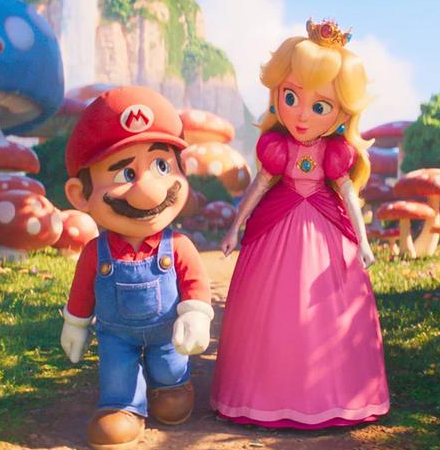
\includegraphics[width=0.3\linewidth]{4x1-pythagore/pb4-mario.png}
  \end{figure}

  \begin{figure}[H]
    \centering
    \includegraphics[width=0.6\linewidth]{4x1-pythagore/pb4.pdf}
  \end{figure}
\end{multicols}

Mario souhaite sauver la princesse Peach. Elle est prisonnière en haut d'une de 45m. Pour cela, il jette un grappin par dessus les douves qui ont une longueur de 35m. 
  
\textbf{Calculer la longueur nécessaire du grappin.} \\

\begin{multicols}{2} 
  \textbf{Problème 3 - Zelda} \\

  \begin{figure}[H]
    \centering
    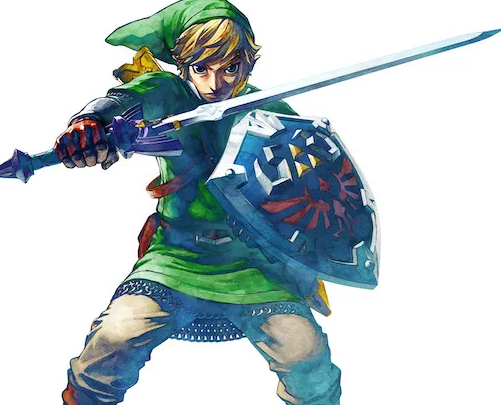
\includegraphics[width=0.5\linewidth]{4x1-pythagore/pb1-link.png}
  \end{figure}

  Dans Zelda, Link doit réparer la voile triangulaire de son bateau. Pour cela, il doit coudre un fils le long des trois côtés du triangle. 

  \textbf{Calculer le périmètre du triangle formé par la voile.} \columnbreak

  \begin{figure}[H]
    \centering
    \includegraphics[width=0.7\linewidth]{4x1-pythagore/pb2-iea.pdf}
  \end{figure}

\end{multicols}

\textbf{Problème 4 - Street fighter} \\

\begin{figure}[H]
  \centering
  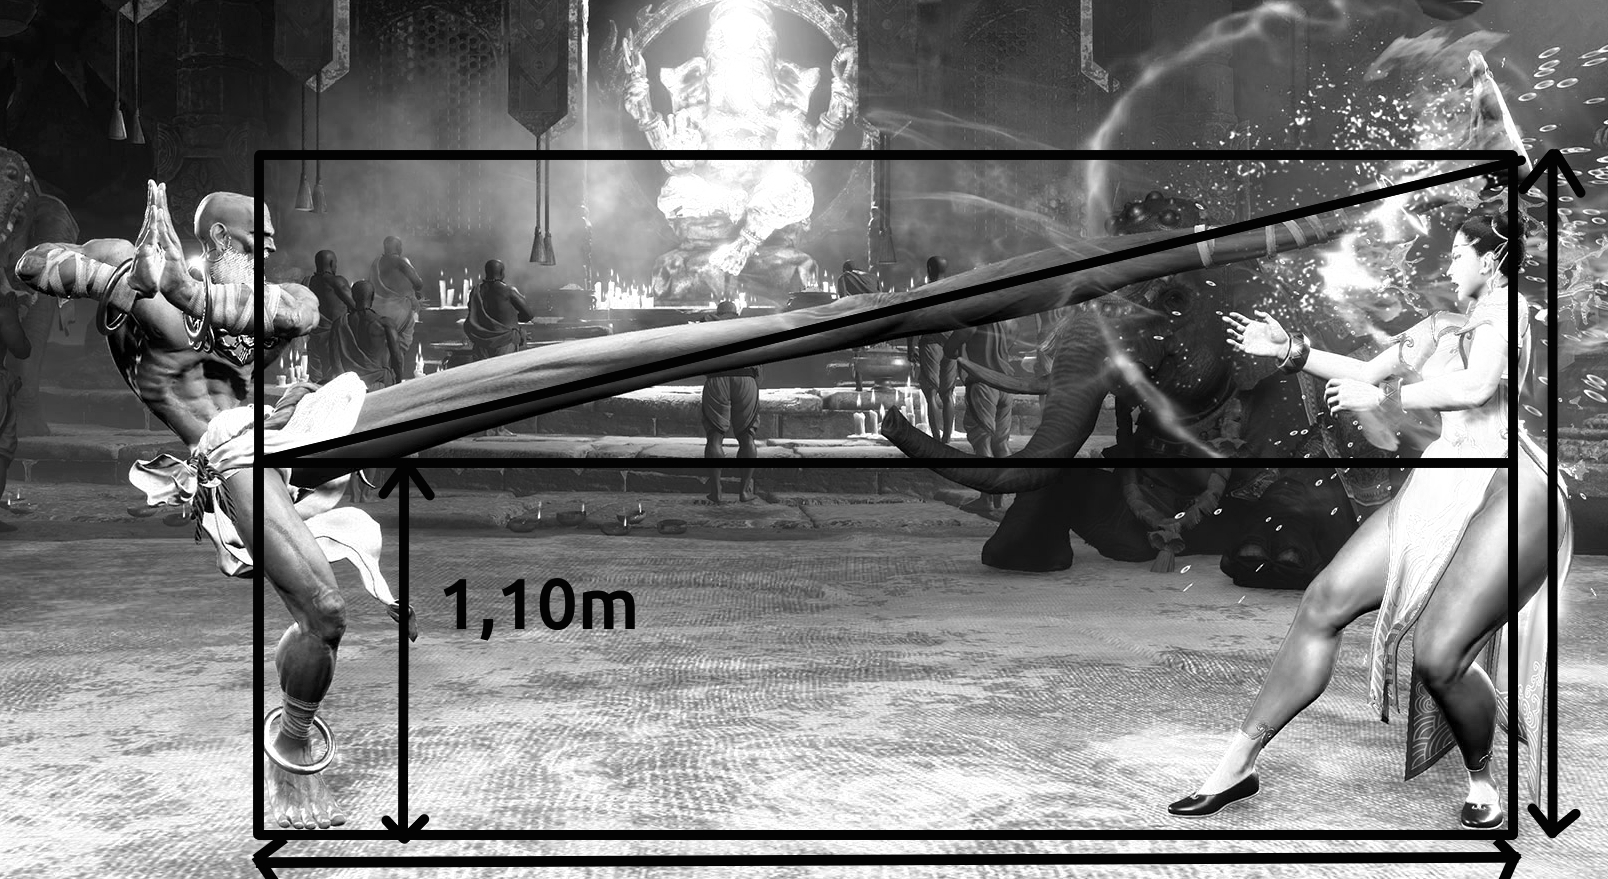
\includegraphics[width=0.5\linewidth]{4x1-pythagore/sf4.jpg}
\end{figure}

Les deux personnages sont perpendiculaires au sol. Dans Street fighter 4, Chun-Li mesure $1,78m$ et Dhalsim mesure $2,05m$. La jambe gauche de Dhalsim mesure $1,10m$ et il est positionné à $3,80m$ de Chun-Li. Lorsqu'il donne un coup du pied gauche, il atteint le haut de sa tête. 

\textbf{Calculer la taille de la jambe gauche de Dhalsim.} 

\newpage

\textbf{Nom, Prénom :} \hspace{8cm} \textbf{Classe :} \hspace{3cm} \textbf{Date :}\\

\begin{center}
  \textit{Le plus grand ennemi de la connaissance n'est pas l'ignorance. C'est l'illusion de la connaissance.} 
  
  \textbf{Stephen Hawking}
\end{center}

\begin{multicols}{2}

\textbf{Ex1 - Calculer} - \textit{Faire les tableaux}\\

Les triangles sont rectangles. \\ 

À l'aide du théorème de Pythagore, faire les tableaux et trouver les longueurs manquantes. \columnbreak

\begin{figure}[H]
  \centering
  \includegraphics[width=0.7\linewidth]{4x1-pythagore/ex1-ieb.pdf}
\end{figure} 

\end{multicols} 

\textbf{Ex2 - Égalité de Pythagore} - \textit{Écrire les égalités de Pythagore.}\\

\begin{itemize}
  \item[1.] Le triangle $IBM$ est rectangle en $M$. 
  \item[2.] Le triangle $DOS$ est rectangle en $D$. \\
\end{itemize}

\textbf{Ex3 - Rédaction} - \textit{Rédiger l'exercice de Pythagore}\\

\begin{enumerate}
  \item[1.] Le triangle $PGM$ est rectangle en $M$. On a $MG = 22cm$ et $MP = 32cm$. Calculer $PG$. 
  \item[2.] Le triangle $LOW$ est rectangle en $O$. On a $OL = 63cm$ et $OW = 71cm$. Calculer $LW$. \\
\end{enumerate} 

\textbf{Problème 1 - FIFA 2025} \\

\begin{figure}[H]
  \centering
  \includegraphics[width=0.4\linewidth]{4x1-pythagore/pb3.pdf}
\end{figure}
  
Pour gagner votre match sur FIFA 2025, vous suivez la formation du triangle rectangle en attaque. Le triangle VMB formé par Vinicius Jr, Mbappé et le But est rectangle en B. \\
  
Mbappé fait la passe a Vinicius Jr qui marque une sublime reprise de volée. 
  
\begin{itemize}
  \item Distance entre Vinicius Jr et le But : $VB = 14m$
  \item Distance entre Mbappé et le But : $PB = 17m$
\end{itemize}
  
\textbf{Calculer la distance VM entre Vinicius Jr et Mbappé.} 

\newpage

\begin{multicols}{2} 
  \textbf{Problème 2 - Mario} \\
  
  \begin{figure}[H]
    \centering
    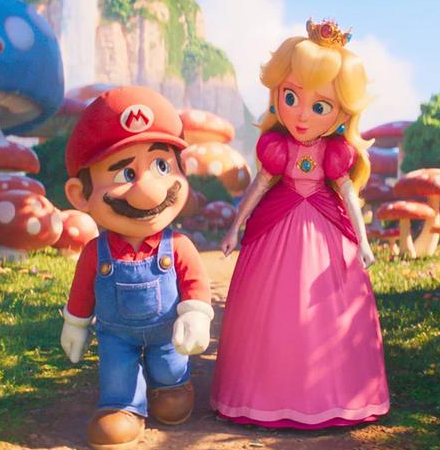
\includegraphics[width=0.3\linewidth]{4x1-pythagore/pb4-mario.png}
  \end{figure}

  \begin{figure}[H]
    \centering
    \includegraphics[width=0.6\linewidth]{4x1-pythagore/pb4.pdf}
  \end{figure}
\end{multicols}

Mario souhaite sauver la princesse Peach. Elle est prisonnière en haut d'une de 42m. Pour cela, il jette un grappin par dessus les douves qui ont une longueur de 32m.
  
\textbf{Calculer la longueur nécessaire du grappin.} \\

\begin{multicols}{2} 
  \textbf{Problème 3 - Zelda} \\

  \begin{figure}[H]
    \centering
    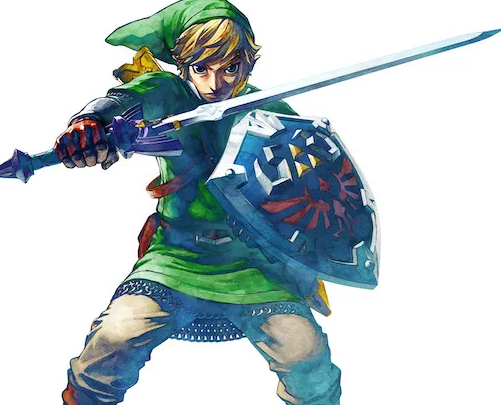
\includegraphics[width=0.5\linewidth]{4x1-pythagore/pb1-link.png}
  \end{figure}

  Dans Zelda, Link doit réparer la voile triangulaire de son bateau. Pour cela, il doit coudre un fils le long des trois côtés du triangle. 

  \textbf{Calculer le périmètre du triangle formé par la voile.} \columnbreak

  \begin{figure}[H]
    \centering
    \includegraphics[width=0.7\linewidth]{4x1-pythagore/pb2-ieb.pdf}
  \end{figure}

\end{multicols}

\textbf{Problème 4 - Street fighter} \\

\begin{figure}[H]
  \centering
  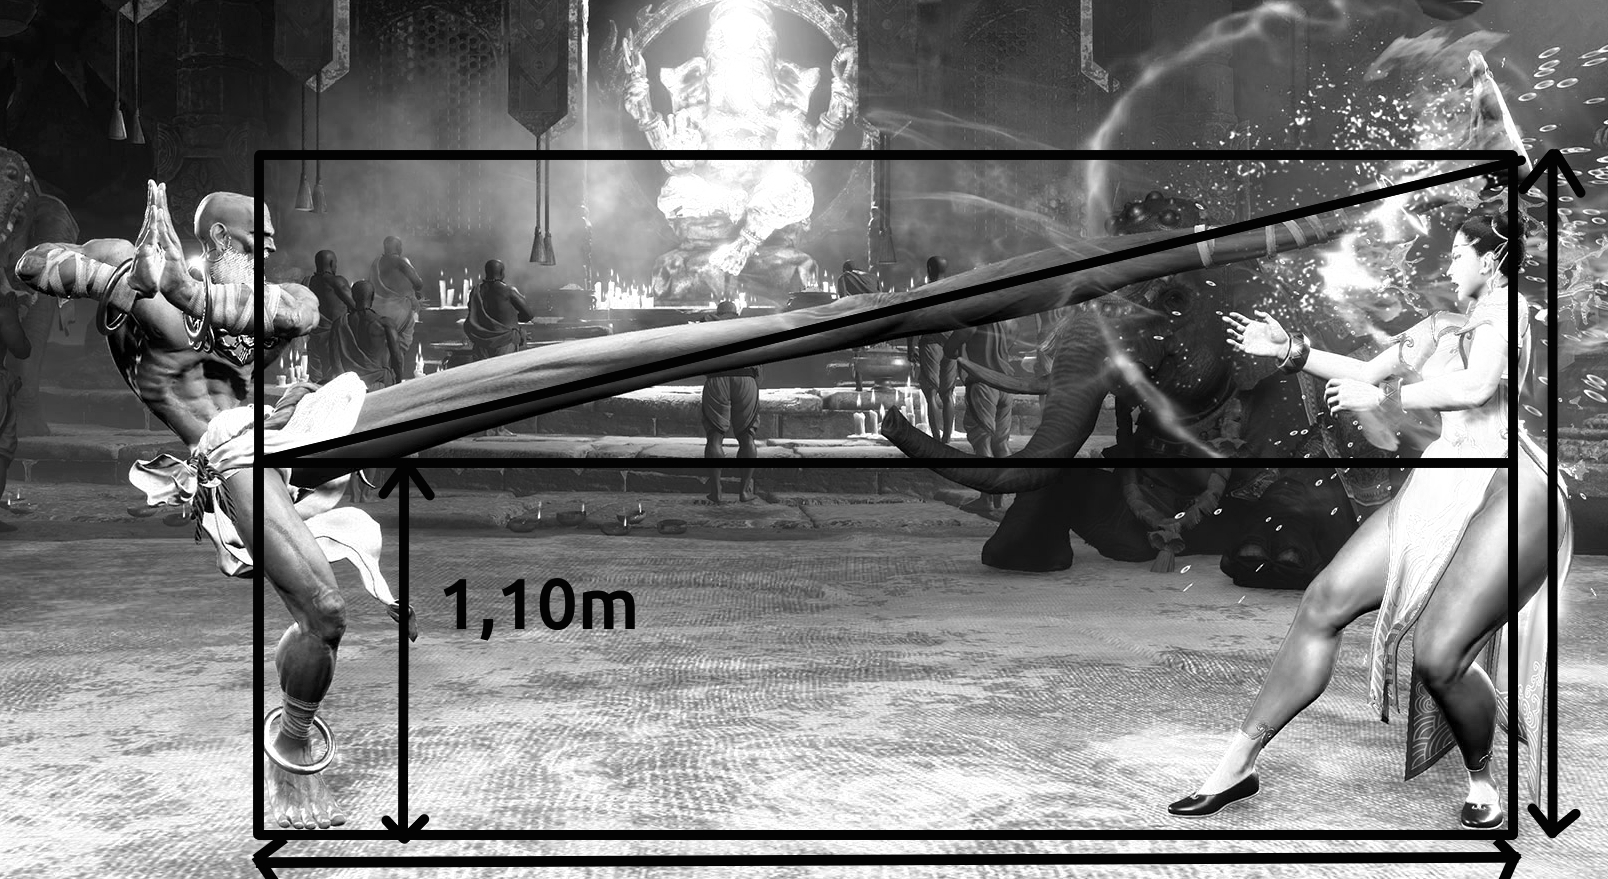
\includegraphics[width=0.5\linewidth]{4x1-pythagore/sf4.jpg}
\end{figure}

Les deux personnages sont perpendiculaires au sol. Dans Street fighter 4, Chun-Li mesure $1,76m$ et Dhalsim mesure $2,01m$. La jambe gauche de Dhalsim mesure $1,05m$ et il est positionné à $4,10m$ de Chun-Li. Lorsqu'il donne un coup du pied gauche, il atteint le haut de sa tête. \\

\textbf{Calculer la taille de la jambe gauche de Dhalsim.} 

\end{document}